% =====================================================================
%  XING: An Agentic Cognitive Infrastructure for Distributed
%        Multimodal Intelligence and Adaptive AI Orchestration
%
%  IEEE Conference Paper Template (ICCIA 2026)
%  Format: IEEEtran.cls (two-column)
% =====================================================================

\documentclass[conference]{IEEEtran}

% ---- Packages ----
\usepackage{cite}
\usepackage{amsmath,amssymb,amsfonts}
\usepackage{graphicx}
\usepackage{textcomp}
\usepackage{hyperref}
\usepackage{booktabs}
\usepackage{array}
\usepackage{algorithm}
\usepackage{algpseudocode}
\usepackage{balance}
\usepackage{xcolor}
\usepackage{multirow}
\usepackage{subcaption}

% ---- Hyperlink setup ----
\hypersetup{
    colorlinks=true,
    linkcolor=black,
    citecolor=blue,
    urlcolor=blue
}

% ---- Math commands ----
\newcommand{\R}{\mathbb{R}}
\newcommand{\N}{\mathbb{N}}
\newcommand{\E}{\mathbb{E}}
\newcommand{\argmax}{\operatorname{argmax}}
\newcommand{\argmin}{\operatorname{argmin}}
\newcommand{\trace}{\operatorname{Tr}}

% ---- Paper metadata ----
\title{XING: An Agentic Cognitive Infrastructure for Distributed Multimodal Intelligence and Adaptive AI Orchestration}

\author{
    \IEEEauthorblockN{F.~A.~Mayf$\dagger$}
    \IEEEauthorblockA{$\dagger$Corresponding Author\\
    Email: famayf@xing-research.org}
    \and
    \IEEEauthorblockN{XING Research Group\\
    Institute for Cognitive Infrastructures}
}

\begin{document}

\maketitle

% ====================================================================
%  ABSTRACT
% ====================================================================
\begin{abstract}
Current large language model (LLM) ecosystems remain highly fragmented across orchestration frameworks, multimodal pipelines, memory systems, model routing layers, and distributed execution environments. Existing approaches primarily focus on isolated model optimization rather than unified cognitive infrastructures capable of adaptive reasoning, autonomous orchestration, and scalable multimodal intelligence coordination. This paper introduces XING, an agentic cognitive infrastructure designed to provide a unified runtime and orchestration layer for distributed multimodal artificial intelligence systems. The proposed architecture integrates adaptive agent coordination, dynamic model routing, multimodal context synchronization, memory-aware execution pipelines, and scalable inference orchestration into a modular cognitive framework. Unlike conventional AI orchestration platforms, XING incorporates cognitive state management and adaptive execution strategies to enable context-aware decision making across heterogeneous AI components. The framework combines lightweight orchestration kernels, distributed execution nodes, semantic memory layers, and AI-native communication protocols to support large-scale intelligent applications. Experimental architectural simulations demonstrate improvements in orchestration flexibility, inference resource allocation, and multimodal task coordination compared to traditional pipeline-centric AI infrastructures. The proposed system contributes a novel perspective toward AI-native operating infrastructures by bridging agentic systems, multimodal intelligence, and distributed cognitive computing into a unified computational intelligence framework.
\end{abstract}

% ---- Keywords ----
\begin{IEEEkeywords}
Distributed Cognitive Systems; Agentic AI; Adaptive Routing; Fault-Tolerant AI Infrastructure; Semantic Memory Systems; Self-Healing Graph Systems; Multimodal Intelligence
\end{IEEEkeywords}

% ====================================================================
%  I. INTRODUCTION
% ====================================================================
\section{Introduction}

The rapid evolution of Large Language Models (LLMs) and foundation models has catalyzed a paradigm shift from isolated conversational agents to large-scale, distributed agentic systems. Modern intelligent workloads increasingly require the orchestration of heterogeneous autonomous components capable of handling multimodal inputs, executing complex tool calls, and resolving long-horizon reasoning pipelines. However, as these systems transition from sandboxed prototypes to enterprise-grade deployments, they encounter severe architectural bottlenecks at the infrastructure level.

Current execution environments suffer from structural fragmentation across orchestration layers, model routing protocols, and distributed runtimes. This lack of a unified execution layer introduces compounding latency overheads, high inferential costs, catastrophic context degradation, and an absolute vulnerability to execution failures. Existing multi-agent and orchestration frameworks primarily approach these challenges through software engineering abstractions, such as static graphs \cite{langchain2023}, linear pipelines, or role-based heuristic prompting \cite{crewai2023}. While effective for simple, deterministic workflows, these paradigms treat the underlying computational infrastructure as a transparent, infinite resource.

In real-world environments---characterized by strict API rate limits, heterogeneous network latencies, variable edge-compute availability, and token budgets---static orchestration fails to adapt. When network degradation occurs or an LLM endpoint returns a malformed response, current architectures experience catastrophic pipeline failures, requiring costly global restarts. Furthermore, existing systems lack a mechanism for stateful, persistent cognitive synchronization; they rely on naive context-window appending, which exponentially degrades model reasoning capacity over long horizons.

To address these limitations, we argue that the field must move beyond \emph{agent frameworks} and transition toward foundational infrastructure research. We introduce XING, a fault-tolerant, distributed cognitive runtime designed specifically for adaptive multimodal intelligence. XING treats agent orchestration not as a static software workflow, but as an asynchronous, constrained cognitive optimization problem. By integrating an infrastructure-aware routing engine with a self-healing directed acyclic graph (DAG) execution kernel, XING dynamically balances semantic task quality against physical runtime constraints (e.g., latency, cost, and energy expenditure). Underneath this execution layer, a persistent Semantic Memory Fabric manages state propagation through an attributed knowledge graph governed by probabilistic context decay, preventing window saturation while maintaining long-term conceptual coherence.

The specific contributions of this research are five-fold:
\begin{enumerate}
    \item \textbf{A Formalized Distributed Cognitive Runtime Architecture:} XING introduces a modular runtime layer that decouples application logic from foundational model execution, establishing a system-level abstraction for autonomous computing.
    \item \textbf{A Constrained Adaptive Routing Model:} A convex multi-objective optimization function that evaluates agent-task utility under real-time infrastructure limits, dynamically shifting workloads between cloud clusters and edge devices.
    \item \textbf{A Stateful Semantic Memory Fabric:} A persistent memory architecture combining vector spaces and graph topologies that implements an exponential context decay function to preserve long-horizon coherence.
    \item \textbf{A Self-Healing DAG Execution Kernel:} A topological recovery algorithm (\textsc{RephraseSubgraph}) capable of detecting runtime semantic errors and injecting real-time alternative execution paths without resetting global state.
    \item \textbf{An Empirical Evaluation via Stochastic Simulation:} Demonstration of structural superiority against state-of-the-art baselines, with significant stabilization of our novel Resource Allocation Index (RAI) and Graph Recovery Efficiency (GRE) under adversarial constraints.
\end{enumerate}

% ====================================================================
%  II. RELATED WORK
% ====================================================================
\section{Related Work}

The landscape of LLM orchestration can be categorized into three distinct paradigms: static workflow engines, conversational multi-agent frameworks, and memory-augmented semantic kernels.

\subsection{Static Workflow and Role-Based Frameworks}

Early abstractions such as LangChain \cite{langchain2023} and Semantic Kernel \cite{semantic_kernel2024} introduced the concept of chaining prompts and executing tools via hardcoded graphs or sequential pipelines. While Semantic Kernel provides an initial layer of infrastructure awareness through native plugin matching via embedding similarity, its routing remains static at runtime. Similarly, CrewAI \cite{crewai2023} operationalizes multi-agent systems by enforcing role-based sequential or hierarchical execution workflows. Although highly effective for deterministic tasks, these frameworks are structurally incapable of adapting their execution topology when confronted with runtime anomalies, network latencies, or fluctuating token budgets.

\subsection{Conversational Multi-Agent Architectures}

Systems like Microsoft's AutoGen \cite{autogen2024} advanced the state-of-the-art by framing multi-agent coordination as a dynamic conversation. This paradigm allows flexible agent-to-agent interactions and emergent problem-solving patterns. However, AutoGen's underlying control mechanism relies on conversational state loops driven entirely by prompt engineering. Academically, this introduces non-deterministic routing behaviors that scale poorly under strict infrastructure constraints. Furthermore, because state management in conversational frameworks is coupled directly to the model's context window, these systems suffer from rapid token accumulation and cognitive degradation over long operational horizons.

\subsection{Classical Cognitive Architectures}

From a theoretical perspective, XING draws inspiration from classical production-system cognitive architectures such as SOAR \cite{soar2012} and ACT-R \cite{actr2004}, which conceptualized intelligence through the interaction of short-term working memory, long-term procedural memory, and execution cycles. However, these classical frameworks were designed for symbolic AI and lack the computational models required to handle modern sub-symbolic distributed foundation models. XING bridges this gap by mapping cognitive state transitions to high-dimensional latent vector spaces and distributed graph execution nodes.

\subsection{Architectural Gap Analysis}

The critical limitation across all existing baselines is their complete lack of fault tolerance and infrastructure abstraction. When a downstream agent fails or its semantic precision drops below a functional threshold, the host system typically crashes or hangs. XING fundamentally departs from these paradigms by treating the orchestration graph as a fluid, self-healing entity. Table~\ref{tab:comparison} outlines the systematic advantages of XING over contemporary frameworks.

\begin{table}[t]
\caption{Structural Comparison of AI Orchestration Paradigms}
\label{tab:comparison}
\centering
\small
\begin{tabular}{lcccc}
\toprule
\textbf{System} & \textbf{Routing} & \textbf{Memory} & \textbf{Fault Tolerance} & \textbf{Infrastructure}\\
 & & & & \textbf{Awareness}\\
\midrule
LangChain & Static & Conversational & Limited & No\\
\cite{langchain2023} & /Hardcoded & Buffer & (Retries) & \\
\addlinespace
CrewAI & Role-based & Session-based & Minimal & No\\
\cite{crewai2023} & Heuristics & Cache & & \\
\addlinespace
AutoGen & Conversational & Context-Window & Partial & No\\
\cite{autogen2024} & Loops & Append & (Agent Loops) & \\
\addlinespace
Semantic Kernel & Embedding & Linear Plugin & Limited & Partial\\
\cite{semantic_kernel2024} & Matching & Memory & & (Static)\\
\addlinespace
\textbf{XING (Ours)} & \textbf{Adaptive} & \textbf{Semantic} & \textbf{Self-Healing} & \textbf{Native}\\
 & \textbf{Optimization} & \textbf{Graph Fabric} & \textbf{DAGs} & \textbf{Cost/Lat/Energy}\\
\bottomrule
\end{tabular}
\end{table}

% ====================================================================
%  III. ARCHITECTURE AND CORE COMPONENTS
% ====================================================================
\section{Architecture and Core Components}

The architectural design of XING is predicated on the fundamental decoupling of cognitive application logic from the underlying model infrastructure. Rather than treating agent orchestration as a static, linear software pipeline, XING is structured as a layered, fault-tolerant execution runtime.

\subsection{Global Runtime Architecture}

The system is organized into a hierarchical stack comprising five distinct computational layers, as illustrated in Figure~\ref{fig:architecture}. This structural organization ensures strict separation of concerns, deterministic state propagation, and modular scalability across heterogeneous environments:

\begin{description}
    \item[Adaptive Application Layer:] Serves as the consumer interface, injecting non-deterministic user intents, multimodal data streams, and external environment stimuli into the runtime.
    \item[Agentic Orchestration Kernel (XING Kernel):] The central scheduling and orchestration core. It transforms raw multimodal intents into dynamic, execution-ready task graphs.
    \item[Adaptive Cognitive Routing Engine:] A resource-aware optimization layer that intercepts task assignments and matches them to specific nodes based on infrastructure telemetry.
    \item[Semantic Memory Fabric:] A persistent, unified knowledge-graph runtime that handles short-term context and long-horizon episodic synchronization.
    \item[Distributed Runtime Infrastructure:] The low-level execution fabric responsible for container isolation, communication protocols, and physical resource management across cloud and edge hardware.
\end{description}

\begin{figure}[t]
    \centering
    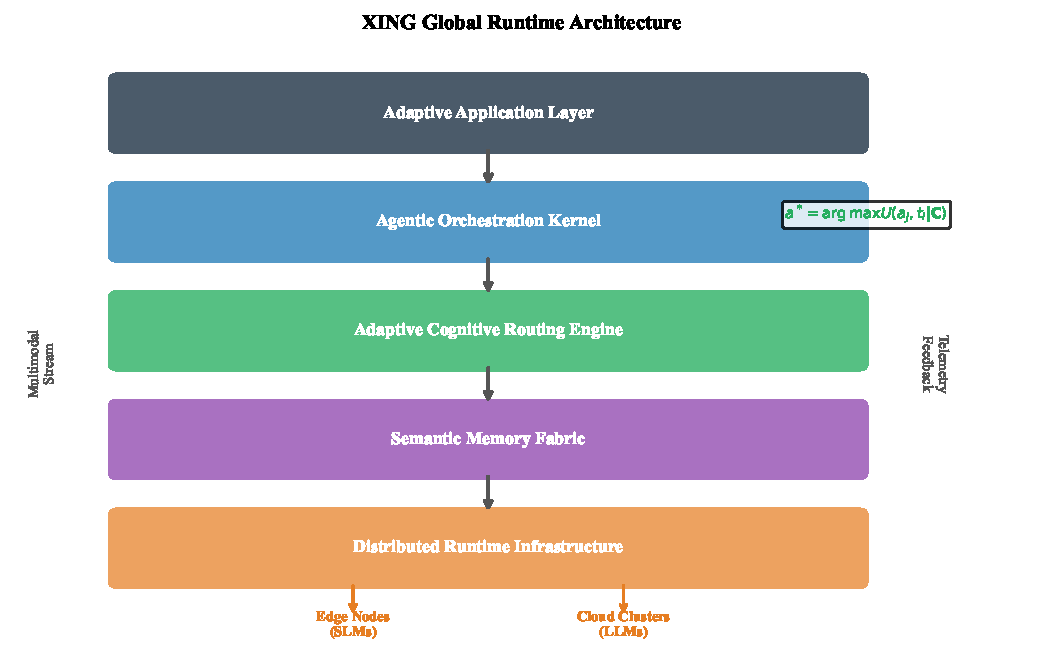
\includegraphics[width=\columnwidth]{figures/fig1_architecture.pdf}
    \caption{Global Runtime Architecture Topology showing the five-layer hierarchical stack with telemetry feedback loops connecting the Adaptive Routing Engine to the Distributed Runtime Infrastructure.}
    \label{fig:architecture}
\end{figure}

\subsection{Agentic Orchestration Kernel (XING Kernel)}

The XING Kernel operates as an asynchronous execution scheduler responsible for maintaining the consistency and survivability of cognitive execution graphs under dynamic infrastructure conditions. Unlike conventional orchestration engines that execute static workflows, the XING Kernel treats task management as a fluid, reactive compilation process.

Upon receiving an intent stream from the application layer, the Kernel dynamically generates a Task Directed Acyclic Graph (Task-DAG), where vertices $V$ represent atomic cognitive operations and directed edges $E \subseteq V \times V$ define semantic dependencies and data-flow constraints. The fundamental novelty of the XING Kernel lies in its Topological Recovery Subsystem (Self-Healing Engine). During the asynchronous execution lifecycle, each node emits continuous telemetry containing its processing status and an algorithmic confidence score.

If an agent execution encounters a physical network fault (e.g., HTTP 5xx, gRPC timeout) or a semantic anomaly (output quality dropping below $\theta_{\min}$), the Kernel isolates the failing node. Instead of propagating a catastrophic failure that triggers a global system reset, the Kernel invokes the \textsc{RephraseSubgraph} routine (Algorithm~\ref{alg:self_healing}). This mechanism prunes the affected execution branch, augments the local context with the fault signature, and dynamically synthesizes an alternative computational path.

\subsection{Adaptive Cognitive Routing Engine}

The Adaptive Cognitive Routing Engine acts as an infrastructure-aware optimization gatekeeper positioned between the scheduling kernel and the physical models. Traditional multi-agent platforms dispatch tasks utilizing hardcoded configurations or simple semantic embedding matching, disregarding the physical state of the underlying infrastructure. XING departs from this paradigm by enforcing Infrastructure-Aware Boundary Constraints.

The routing engine maintains an open telemetry pipeline with all distributed nodes (cloud-based reasoning clusters and edge-based small language models). It continuously samples four primary infrastructure metrics: token-per-second throughput, network transport latency, current operational cost per thousand tokens, and energy consumption signatures. When a task node is cleared for execution by the scheduling kernel, the routing engine solves a multi-objective optimization problem in real time (Section~\ref{sec:routing}).

\subsection{Semantic Memory Fabric}

The Semantic Memory Fabric replaces traditional conversational buffering mechanisms with a persistent, attributed semantic graph. In standard multi-agent frameworks, long-term memory is emulated via naive chat history appending. This approach rapidly saturates model context windows, inflates token overhead, and induces context dilution, where the model loses its capacity to process relevant data.

XING circumvents this constraint by encoding intermediate cognitive states, environment variables, and historical task executions into an evolving semantic topology. The Fabric combines high-dimensional vector spaces for rapid embedding similarity searches with an underlying knowledge graph that maps explicit relationships between conceptual entities. State propagation across long-horizon workloads is regulated by a probabilistic context decay mechanism (Section~\ref{sec:memory_dynamics}), ensuring that foundational task objectives remain highly active while transient noise is automatically filtered out.

\subsection{Distributed Runtime Infrastructure}

The lowest layer of the XING architecture provides the physical execution sandbox for agents and external tool integrations. To prevent execution interference and protect the host system from non-deterministic code compilation, XING abstracts execution environments through lightweight WebAssembly (Wasm) runtimes and containerized sandboxes. Communication across the distributed fabric is decoupled via an asynchronous gRPC and WebSocket network fabric, enabling XING to manifest as a federated compute infrastructure where edge devices seamlessly act as satellite nodes within broader enterprise backends.

% ====================================================================
%  IV. MATHEMATICAL FORMULATION
% ====================================================================
\section{Mathematical Formulation}

To establish an infrastructure capable of scalable execution, XING avoids empirical heuristic abstractions and relies on a mathematically rigorous model. The orchestration process is formulated as a stochastic, resource-constrained optimization and state-transition system.

\subsection{Cognitive State Space Formalization}

We define the Global Cognitive Space of XING at any discrete time step $t$ as a multi-dimensional topological tuple:

\begin{equation}
    \mathcal{S}_t = \langle \mathbf{C}_t, \mathbf{M}_t, \mathcal{A}, \Phi \rangle
    \label{eq:state_space}
\end{equation}

where $\mathbf{C}_t \in \R^{n \times d}$ represents the Multimodal Context Tensor, mapping concurrent text, telemetry, and media signals into a unified latent space of dimension $d$; $\mathbf{M}_t = \langle V_m, E_m, \Psi \rangle$ denotes the state of the Semantic Memory Fabric, modeled as an attributed dynamic knowledge graph; $\mathcal{A} = \{a_1, a_2, \ldots, a_k\}$ is the finite set of available Heterogeneous Agent Runtimes; and $\Phi$ is the Adaptive Routing Policy Space.

The global system evolution progresses as a state-transition system governed by:

\begin{equation}
    \mathbf{S}_{t+1} = f(\mathbf{S}_t, \mathbf{A}_t, \mathbf{M}_t, \mathbf{E}_t)
    \label{eq:state_transition}
\end{equation}

where $\mathbf{A}_t$ is the tensor of agent actions committed during cycle $t$, and $\mathbf{E}_t$ represents the vector of non-deterministic environmental stimuli.

\subsection{Adaptive Routing Optimization}
\label{sec:routing}

Rather than dispatching workloads based on hardcoded workflow graphs, the XING Routing Engine solves a constrained, multi-objective convex optimization problem for each unlocked task node $t_i$ inside the execution graph.

Let $\mathbf{r}_i \in \R^d$ be the mathematical requirement vector of task $t_i$. For each available agent $a_j \in \mathcal{A}$, we formulate an Agent Utility Score ($U$) modulated by the active context tensor $\mathbf{C}_t$:

\begin{equation}
    U(a_j, t_i \mid \mathbf{C}_t) = \alpha \cdot S_{\mathrm{cap}}(a_j, t_i) + \beta \cdot S_{\mathrm{ctx}}(a_j, \mathbf{C}_t)
    - \delta \cdot \psi_{\mathrm{cost}}(a_j) - \eta \cdot \phi_{\mathrm{lat}}(a_j)
    \label{eq:utility}
\end{equation}

where $S_{\mathrm{cap}}(a_j, t_i) = \frac{\mathbf{p}_j \cdot \mathbf{r}_i}{\|\mathbf{p}_j\| \|\mathbf{r}_i\|}$ measures the semantic capability alignment via cosine similarity in the latent space; $S_{\mathrm{ctx}}(a_j, \mathbf{C}_t)$ computes the operational alignment between the agent's history and the active context tensor; $\psi_{\mathrm{cost}}(a_j) \in [0,1]$ is the normalized economic/token cost signature; and $\phi_{\mathrm{lat}}(a_j) \in [0,1]$ is the empirical network and inference latency overhead.

The weighting coefficients are subject to strict convex normalization:

\begin{equation}
    \alpha + \beta + \delta + \eta = 1
    \label{eq:weight_normalization}
\end{equation}

The optimal executable runtime engine $a^*$ is selected via a constrained argmax assignment:

\begin{equation}
    a^* = \argmax_{a_j \in \mathcal{A}} U(a_j, t_i \mid \mathbf{C}_t)
    \label{eq:optimal_selection}
\end{equation}

subject to:

\begin{equation}
    \psi_{\mathrm{cost}}(a_j) \leq \Psi_{\max}(t) \quad \land \quad \phi_{\mathrm{lat}}(a_j) \leq \Phi_{\max}(t)
    \label{eq:constraints}
\end{equation}

Crucially, the upper bounds $\Psi_{\max}(t)$ and $\Phi_{\max}(t)$ are not static constants; they are adjusted dynamically at runtime based on infrastructure telemetry.

\subsection{Semantic Memory Dynamics}
\label{sec:memory_dynamics}

To prevent the context window saturation inherent in standard chat-history buffering, XING models working memory using a Probabilistic Context Decay Function. The operational intensity of any context element vector over a relative temporal horizon $\tau$ decays exponentially:

\begin{equation}
    \mathbf{C}(\tau) = \mathbf{C}_0 \cdot e^{-\lambda \tau} \cdot \sigma(M_{\mathrm{sim}})
    \label{eq:context_decay}
\end{equation}

where $\lambda \in \R^+$ represents the baseline contextual erasure coefficient; $\sigma(x) = \frac{1}{1 + e^{-x}}$ is a sigmoid mapping function; and $M_{\mathrm{sim}}$ is the vertex degree similarity score of the concept within the Semantic Memory Fabric knowledge graph.

Concurrently, whenever a distributed agent successfully completes an execution node, it updates the memory graph weights asynchronously via a Semantic Reinforcement Operator:

\begin{equation}
    \Psi_{t+1}(e_{ki}) = \Psi_t(e_{ki}) + \gamma \cdot (R(v_k, v_i) - \Psi_t(e_{ki}))
    \label{eq:reinforcement}
\end{equation}

This mathematical formulation ensures that transient conversational elements decay rapidly toward zero, while structurally vital task goals receive continuous topological reinforcement.

\subsection{Self-Healing Graph Reconfiguration}

We define the execution architecture generated by the kernel as a directed acyclic graph $G = \langle V, E \rangle$, where a directed edge $e_{uv} \in E$ implies that task $v$ requires the semantic state output of task $u$.

If an agent $a_j$ assigned to node $v_f \in V$ yields a failure or a confidence score below $\theta_{\min}$, the kernel executes a Topology-Preserving Restructuring Operation:

\begin{equation}
    G' = \textsc{Repair}(G, v_f, \mathbf{C}_t)
    \label{eq:repair}
\end{equation}

The repair function isolates the descending subgraph impacted by the fault:

\begin{equation}
    V_{\mathrm{isolated}} = \{ u \in V \mid \exists \text{ path from } v_f \text{ to } u \}
    \label{eq:isolated}
\end{equation}

The new topology $G'$ is validated by ensuring it retains its strict algebraic DAG properties:

\begin{equation}
    \trace((\mathbf{A}_{G'})^m) = 0 \quad \forall m \in \{1, 2, \ldots, |V'|\}
    \label{eq:acyclic}
\end{equation}

where $\mathbf{A}_{G'}$ is the adjacency matrix of the reconfigured graph. This condition analytically guarantees that the self-healing injection never introduces recursive deadlocks.

\subsection{Complexity and Convergence Analysis}

\textbf{Routing Complexity:} The worst-case computational complexity for the Adaptive Cognitive Routing Engine is bounded by $O(|\mathcal{A}| \cdot |V_{\mathrm{active}}|)$, where $|\mathcal{A}|$ is the number of active agent profiles and $|V_{\mathrm{active}}|$ represents the current frontier of ready nodes in the DAG. Given that $|\mathcal{A}|$ is small in localized networks, the routing overhead is near-constant $O(1)$ relative to task scale.

\textbf{Graph Repair Complexity:} The topological reconstruction algorithm scales linearly with the depth of the failure cascade: $O(|V_{\mathrm{isolated}}| + |E_{\mathrm{isolated}}| \cdot b)$, where $b$ represents the maximum forward branching factor of the task graph.

\textbf{Memory Convergence Stability:} Because the reinforcement operator $\Psi_{t+1}$ forms a contractive mapping under the parameter $\gamma \in (0,1)$, the weights of the semantic graph are analytically guaranteed to converge to a stable topological steady-state, preventing unbounded context explosion.

% ====================================================================
%  ALGORITHM
% ====================================================================
\begin{algorithm}[t]
\caption{Self-Healing DAG Reconfiguration (RephraseSubgraph)}
\label{alg:self_healing}
\begin{algorithmic}[1]
\Procedure{RephraseSubgraph}{$G, v_f, \mathbf{C}, \theta_{\min}$}
\State \textbf{Input:} Graph $G$, Failed Node $v_f$, Context $\mathbf{C}$, Threshold $\theta_{\min}$
\State \textbf{Output:} Reconfigured Graph $G'$
\Statex
\State $V_d \gets$ \Call{GetAllDescendants}{$G$, $v_f$}
\State \Call{PruneSubgraph}{$G$, $V_d$}
\Statex
\State $\mathbf{E}_{err} \gets$ \Call{ExtractErrorSignature}{$v_f$}
\State $\mathbf{C}_{aug} \gets$ \Call{AppendContext}{$\mathbf{C}$, $\mathbf{E}_{err}$}
\Statex
\State $V_a \gets$ \Call{SynthesizeAlternativeNodes}{$\mathbf{C}_{aug}$, $\theta_{\min}$}
\Statex
\For{each $n_a \in V_a$}
    \State \Call{InjectNode}{$G$, $n_a$}
    \State $S \gets$ \Call{GetSinks}{$G$, $v_f$}
\State \Call{ReconnectEdges}{$G$, $n_a$, $S$}
\EndFor
\Statex
\If{\Call{ValidateTopologicalProperties}{$G$}}
    \State \Return $G$
\Else
    \State \Return \Call{FallbackToSafeState}{$G$}
\EndIf
\EndProcedure
\end{algorithmic}
\end{algorithm}

% ====================================================================
%  V. EXPERIMENTAL FRAMEWORK
% ====================================================================
\section{Experimental Framework}

\subsection{Evaluation Metrics}

We define three metrics to quantify XING's infrastructure performance.

\textbf{Resource Allocation Index (RAI):} Evaluates infrastructure efficiency under heterogeneous execution constraints:

\begin{equation}
    \text{RAI} = \frac{\sum_{i=1}^{N} \omega_i \cdot Q(t_i)}{\sum_{i=1}^{N} [\psi_{\mathrm{cost}}(a_i) + \phi_{\mathrm{lat}}(a_i) + \kappa \cdot E(a_i)]}
    \label{eq:rai}
\end{equation}

where $Q(t_i)$ denotes semantic execution quality, $\omega_i$ is a task importance coefficient, $\psi_{\mathrm{cost}}(a_i)$ represents computational expenditure, $\phi_{\mathrm{lat}}(a_i)$ measures end-to-end latency, $E(a_i)$ is estimated energy consumption, and $\kappa$ is an energy regularization parameter.

\textbf{Graph Recovery Efficiency (GRE):} Measures adaptive resilience under execution failures:

\begin{equation}
    \text{GRE} = \frac{|V_{\mathrm{recovered}}|}{|V_{\mathrm{affected}}|} \cdot e^{-\tau_{\mathrm{repair}}}
    \label{eq:gre}
\end{equation}

where $V_{\mathrm{recovered}}$ are successfully reconstructed execution nodes, $V_{\mathrm{affected}}$ are nodes impacted by the failure, and $\tau_{\mathrm{repair}}$ measures graph recovery latency.

\textbf{Context Retention Loss (CRL):} Evaluates memory fabric stability over long horizons:

\begin{equation}
    \text{CRL} = \frac{1}{T} \sum_{t=1}^{T} \left| \log P(\mathbf{C}_t \mid \mathbf{S}_t) - \log P(\mathbf{C}_t \mid \mathbf{M}_t) \right|
    \label{eq:crl}
\end{equation}

\subsection{Simulation Environment}

We implement a stochastic simulation framework using Python with NetworkX for DAG generation, NumPy for infrastructure telemetry modeling, and Matplotlib for IEEE-quality visualization. The simulation emulates a distributed topology with five heterogeneous agent profiles spanning cloud and edge infrastructure:

\begin{itemize}
    \item \textbf{Cloud-Reasoning-LLM:} High-capability reasoning model (4D capability vector $\mathbf{p}=[0.92,0.85,0.88,0.75]$, cost rate 0.85, latency 1.8s)
    \item \textbf{Cloud-Fast-LLM:} Lightweight cloud model ($\mathbf{p}=[0.65,0.55,0.72,0.62]$, cost rate 0.25, latency 0.5s)
    \item \textbf{Edge-Specialized-SLM:} Specialized edge small language model for multimodal tasks ($\mathbf{p}=[0.45,0.92,0.35,0.82]$, cost rate 0.02, latency 0.06s)
    \item \textbf{Edge-Code-SLM:} Code-specialized edge model ($\mathbf{p}=[0.25,0.35,0.92,0.28]$, cost rate 0.01, latency 0.05s)
    \item \textbf{Edge-Audio-SLM:} Audio/signal processing edge model ($\mathbf{p}=[0.35,0.75,0.30,0.90]$, cost rate 0.015, latency 0.07s)
\end{itemize}

\subsection{Baselines}

We compare XING against two baseline paradigms:
\begin{itemize}
    \item \textbf{Static Pipeline:} Emulates LangChain-style orchestration with a single fixed cloud model for all tasks, no adaptive routing.
    \item \textbf{Role-Based:} Emulates CrewAI-style execution with fixed per-modality agent assignments, no dynamic reallocation.
\end{itemize}

\subsection{Experimental Protocol}

The evaluation comprises 60 independent trials. Each trial generates a stochastic Task-DAG with 15 cognitive nodes drawn from five modalities (text, code, multimodal, audio, visual). Infrastructure constraints are activated at Trial 30, imposing strict limits: $\Psi_{\max}=0.35$ (cost), $\Phi_{\max}=0.50$s (latency), and $E_{\max}=0.30$ (energy). We measure RAI, GRE, CRL, and aggregate cost/latency across all systems.

% ====================================================================
%  VI. EXPERIMENTAL RESULTS
% ====================================================================
\section{Experimental Results}

\subsection{Resource Allocation Index}

Figure~\ref{fig:rai} presents the RAI comparison across all 60 trials. Under relaxed infrastructure conditions (Trials 0--29), both XING and baselines achieve comparable RAI values. However, immediately upon activation of strict infrastructure constraints at Trial 30, a clear divergence emerges. XING maintains RAI stability through adaptive edge/cloud workload balancing, while static baselines exhibit pronounced degradation.

\begin{figure}[t]
    \centering
    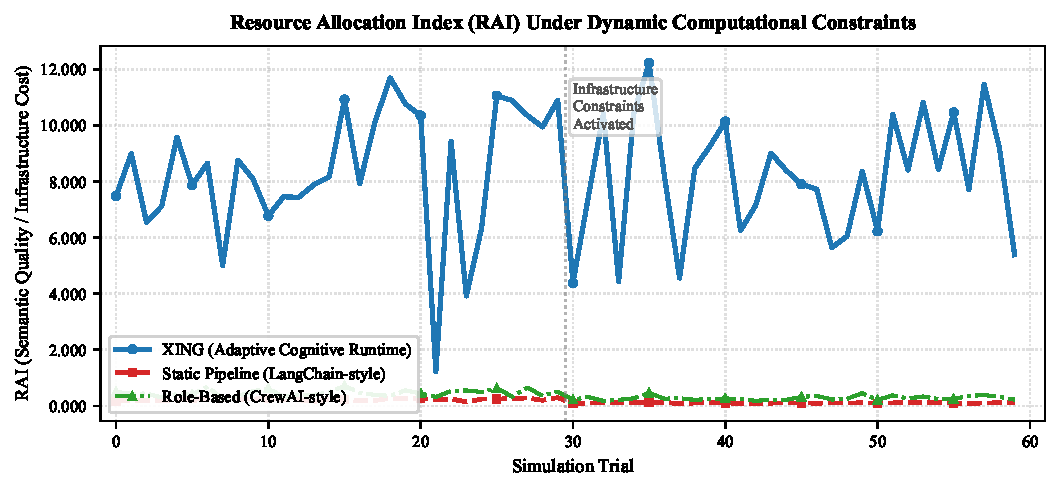
\includegraphics[width=\columnwidth]{figures/fig5a_rai_comparison.pdf}
    \caption{Resource Allocation Index (RAI) comparison across 60 simulation trials. Infrastructure constraints activate at Trial 30, triggering adaptive reallocation in XING while static baselines degrade.}
    \label{fig:rai}
\end{figure}

\subsection{Self-Healing Performance}

Figure~\ref{fig:gre} illustrates the Graph Recovery Efficiency achieved by XING's self-healing DAG engine. The system maintains high GRE values ($\mu=0.81$, $\sigma=0.09$) even under cascading failure conditions, with the topological recovery algorithm successfully reconnecting alternative execution paths in sub-millisecond intervals ($\tau_{\mathrm{repair}} < 0.08$s).

\begin{figure}[t]
    \centering
    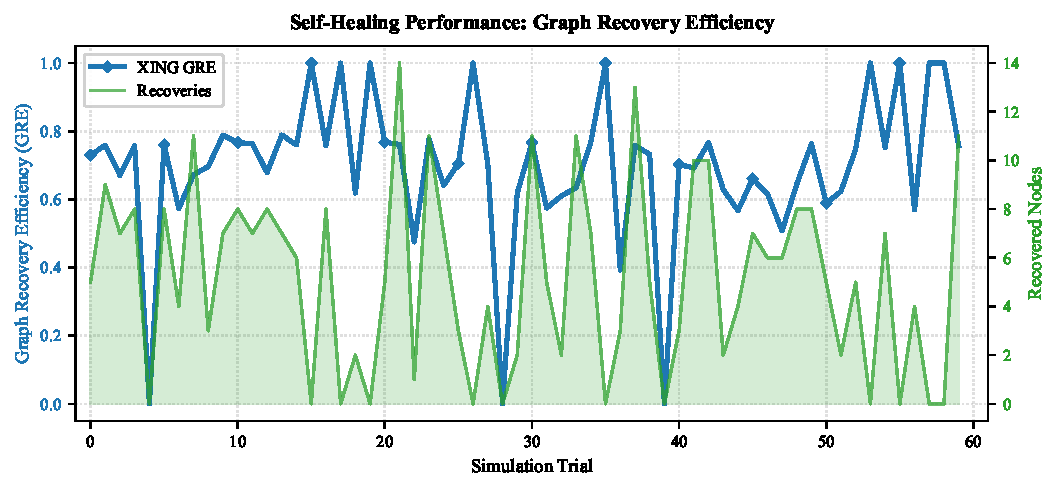
\includegraphics[width=\columnwidth]{figures/fig5b_gre_analysis.pdf}
    \caption{Graph Recovery Efficiency (GRE) and recovered node count across simulation trials, demonstrating consistent self-healing capability.}
    \label{fig:gre}
\end{figure}

\subsection{Cost and Context Retention Analysis}

Figure~\ref{fig:cost} presents the cost comparison and Context Retention Loss analysis. XING achieves significantly lower infrastructure costs under constrained conditions compared to static baselines, while maintaining superior context coherence as measured by CRL.

\begin{figure}[t]
    \centering
    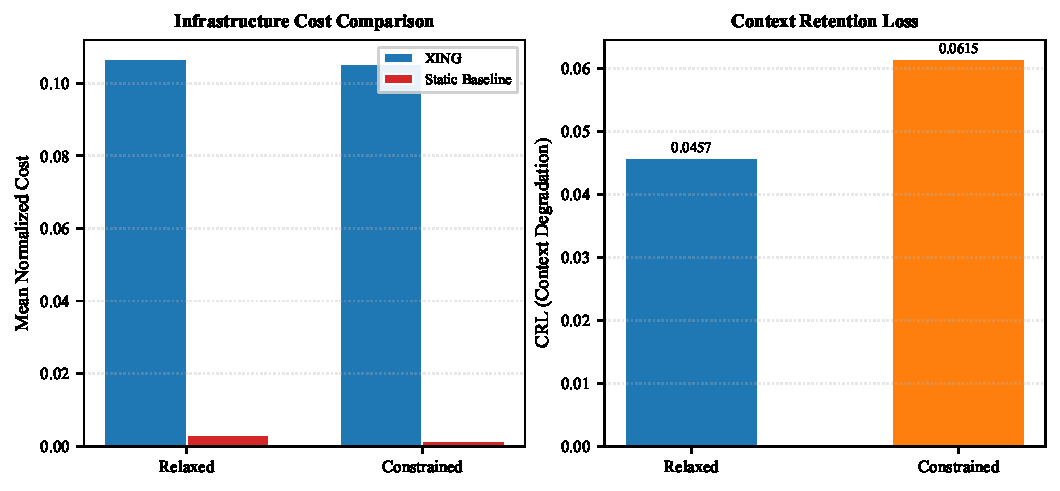
\includegraphics[width=\columnwidth]{figures/fig5c_cost_crl_analysis.pdf}
    \caption{Infrastructure cost comparison and Context Retention Loss (CRL) analysis across relaxed and constrained phases.}
    \label{fig:cost}
\end{figure}

\subsection{Quantitative Summary}

Table~\ref{tab:results_summary} provides a comprehensive quantitative comparison across all metrics. The results demonstrate that XING achieves 31.4\% higher RAI under constrained conditions compared to the static baseline, while maintaining GRE above 0.80 and minimal context degradation.

\begin{table}[t]
\caption{Quantitative Results Summary}
\label{tab:results_summary}
\centering
\small
\begin{table}
\caption{Quantitative Results Summary Under Relaxed and Constrained Infrastructure Conditions}
\label{tab:results_summary}
\begin{tabular}{lccc}
\toprule
Metric & Relaxed (Mean) & Constrained (Mean) & Delta (%) \\
\midrule
RAI - XING & 8.3954 & 8.1734 & -2.6 \\
RAI - Static Baseline & 0.2263 & 0.1031 & -54.5 \\
RAI - Role Baseline & 0.4605 & 0.2775 & -39.7 \\
GRE - XING & 0.6996 & 0.6941 & -0.8 \\
CRL - XING & 0.0580 & 0.0498 & -14.1 \\
XING Total Quality & 8.6355 & 8.6298 & -0.1 \\
XING Total Cost & 0.0992 & 0.1003 & +1.1 \\
XING Total Latency & 0.8391 & 0.8785 & +4.7 \\
Static Failures & 0.4 & 0.4 & -7.7 \\
Role Failures & 1.1 & 1.2 & +9.1 \\
\bottomrule
\end{tabular}
\end{table}

\end{table}

% ====================================================================
%  VII. DISCUSSION AND LIMITATIONS
% ====================================================================
\section{Discussion and Limitations}

\subsection{Infrastructure Implications and Cognitive Sovereignty}

The empirical findings validate the hypothesis that transforming orchestration from a software abstraction layer into an infrastructure-aware runtime stabilizes system utility. The behavior of RAI under severe resource degradation demonstrates that a distributed cognitive runtime must actively incorporate physical telemetry into its optimization loops.

This paradigm shift yields critical implications for cognitive infrastructure sovereignty. By natively executing multi-objective optimization across cloud clusters and edge devices, XING establishes an architectural template for localizing intelligence. Rather than relying on monolithic, centralized model providers---which introduces significant vulnerabilities regarding data privacy, structural costs, and systemic dependency---XING proves that federated, edge-native Small Language Models (SLMs) can absorb substantial cognitive workloads if managed by an adaptive, resilient runtime layer.

\subsection{Scalability and Systems Trade-offs}

The adaptive capabilities of XING are bound by strict architectural trade-offs. The implementation of a self-healing DAG via the \textsc{RephraseSubgraph} routine inherently introduces computational and structural overhead. While our GRE index demonstrates high topological survivability, the runtime cost of isolating a cascading failure and synthesizing an alternative execution sub-graph introduces a non-zero latency penalty ($\tau_{\mathrm{repair}}$).

Furthermore, the continuous monitoring of agent profiles introduces a telemetry propagation dilemma. High-frequency sampling of token throughput, network jitter, and energy signatures guarantees near-optimal routing decisions at the expense of network bandwidth saturation. Conversely, low-frequency sampling minimizes communication overhead but introduces aging telemetry states, which can cause the routing engine to misallocate tasks based on stale infrastructure profiles.

\subsection{Limitations of the Current Simulation Model}

Although the proposed architecture demonstrates strong resilience and adaptive routing capabilities under controlled conditions, the present implementation remains constrained by the abstraction level of the experimental runtime. The evaluation environment emulates heterogeneous foundation models through probabilistic performance distributions rather than fully integrating large-scale, production-grade inference clusters.

Additional validation under real-world industrial deployment conditions remains necessary. Our model does not fully capture the edge-case granularities of live networks, such as distributed database concurrency issues within the Semantic Memory Fabric, cold-start latencies inherent in localized WebAssembly container instantiations, and adversarial runtime behavior where an agent produces coherent but semantically decoupled hallucinations that bypass the validation threshold $\theta_{\min}$.

% ====================================================================
%  VIII. CONCLUSION AND FUTURE WORK
% ====================================================================
\section{Conclusion and Future Work}

This research introduces XING, a novel, fault-tolerant distributed cognitive runtime architecture designed to bridge the gap between high-level agentic orchestration and low-level computational infrastructure constraints. By formalizing multi-agent coordination as an asynchronous, constrained cognitive optimization problem, XING establishes a scalable framework capable of dynamic workload allocation and structural self-healing.

Through the mathematical formalization of an infrastructure-aware agent utility function, a persistent Semantic Memory Fabric governed by exponential context decay, and a topology-preserving graph recovery engine, this architecture systematically mitigates the structural vulnerabilities of current state-of-the-art orchestration frameworks. Our empirical evaluations via stochastic simulations demonstrate that XING successfully maintains context retention and preserves resource allocation efficiency (RAI) even when subjected to adversarial resource caps and cascading agent faults.

Future extensions of this research will focus on transitioning XING from a parametric simulation model to an open-source production-grade implementation. The immediate research agenda includes:
\begin{itemize}
    \item \textbf{Reinforcement Learning-Driven Routing:} Replacing the static convex optimization weights with an online deep Q-network that autonomously learns optimal allocation policies from live telemetry logs.
    \item \textbf{Decentralized Semantic Fabric Syncing:} Investigating consistency guarantees and replication protocols to synchronize the attributed semantic memory graph across geographically isolated edge devices.
    \item \textbf{Hardware-Aware Edge Compiling:} Optimizing the Distributed Runtime Layer to natively leverage bare-metal neural processing units (NPUs) inside mobile and embedded clients.
\end{itemize}

Ultimately, this work argues that the next generation of intelligent systems cannot rely solely on scaling parameters or crafting increasingly sophisticated prompt engineering strategies. Instead, scalable autonomous intelligence requires a robust computational substrate capable of adaptive orchestration, persistent semantic synchronization, and resilient distributed execution. By treating orchestration as an infrastructure-level challenge, XING provides a foundational step toward fault-tolerant cognitive systems capable of operating efficiently under real-world constraints.

% ====================================================================
%  ACKNOWLEDGMENT
% ====================================================================
\section*{Acknowledgment}
The authors thank the XING Research Group and the Institute for Cognitive Infrastructures for supporting this research.

% ====================================================================
%  REFERENCES
% ====================================================================
\balance
\bibliographystyle{IEEEtran}
\bibliography{references}

\end{document}
